
\documentclass[10pt]{amsart}
\usepackage[top=2.5 cm, bottom=2.5 cm, left=1.05in, right=1.05in]{geometry}
\usepackage[section]{placeins}

%\geometry{a4paper} % or letter or a5paper or ... etc
% \geometry{landscape} % rotated page geometry
\usepackage[applemac]{inputenc}
\usepackage{amsmath,amssymb} 
% See the ``Article customise'' template for come common customisations
\usepackage{mathtools}   % loads �amsmath�
\usepackage{listings}

\title{HW6}
\author{Alessandro Manzotti}
\date{} % delete this line to display the current date

%%% BEGIN DOCUMENT
\begin{document}

\maketitle
\section{Problem 1, Perceptron}

Code scripts:
\begin{description}
\item[Kernel online] \texttt{kernel\_perceptron\_online.py}
\item[Kernel batch] \texttt{kernel\_perceptron\_batch.py}
\item[Linear online] \texttt{linear\_perceptron\_online.py}
\item[Linear batch] \texttt{linear\_perceptron\_batch.py}
\item[Kernel test sigma] \texttt{kernel\_perceptron\_online.py}
\item[Linear test run number]\texttt{kernel\_perceptron\_online.py}
\item[Kernel test run number] \texttt{kernel\_perceptron\_run\_batch.py}
\item[Kernel Labels] \texttt{label\_batch\_kernel\_gaussian.txt}
\item[Linear Labels] \texttt{label\_batch\_linear.txt}

\end{description}

\begin{figure}[htbp]
\begin{center}
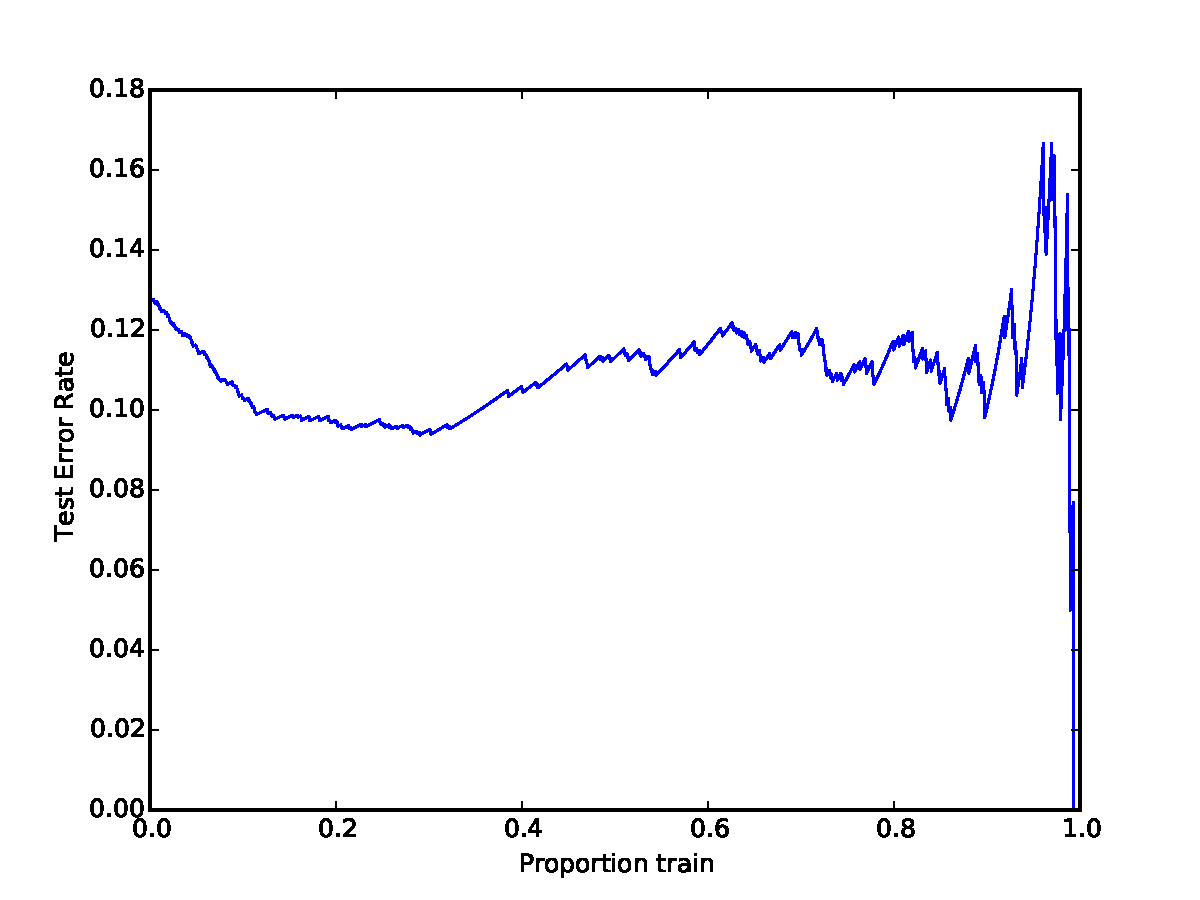
\includegraphics[scale=0.5]{linear_online.pdf}
\caption{Linear perceptron. Number of mistakes (rate) as a function of the example seeen. The percetron is initialized so that $\mathbf{w} = x[0]$ where $x[0]$ is the first training point. This was not done holding a test set from the data. I trained the perceptron online on the data recording the errors made. I did not run different initialized run so this curves are noisy and in particular the tail where we are just looking at the number of errors in the last few points of the data.}
\label{default}
\end{center}
\end{figure}

\begin{figure}[htbp]
\begin{center}
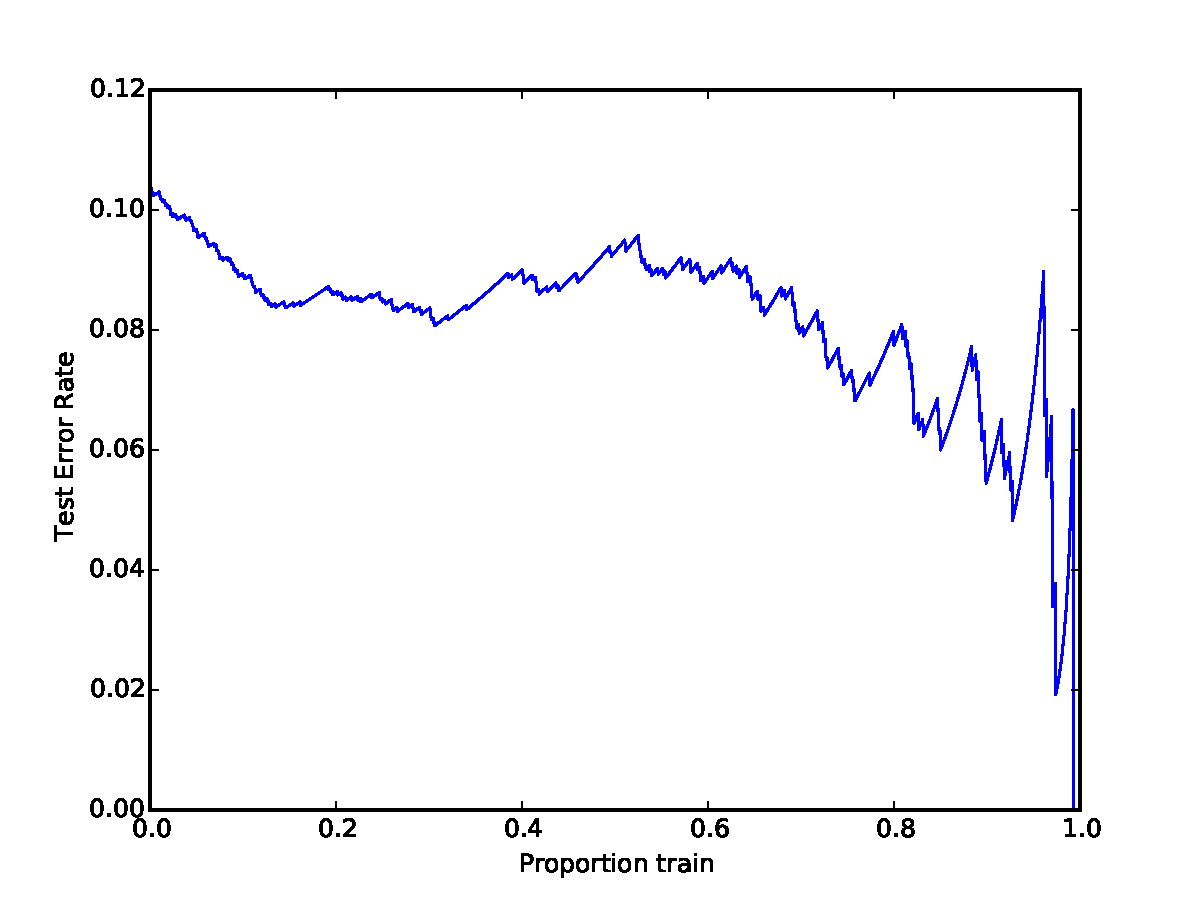
\includegraphics[scale=0.5]{kernel_linear_online.pdf}
\caption{RBF Gaussian with $\sigma=1$. Number of mistakes (rate) as a function of the example seeen. The percetron is initialized so that $\mathbf{w} = x[0]$ where $x[0]$ is the first training point. This was not done holding a test set from the data. I trained the perceptron online on the data recording the errors made. I did not run different initialized run so this curves are noisy and in particular the tail where we are just looking at the number of errors in the last few points of the data.}
\label{default}
\end{center}
\end{figure}



\begin{figure}[htbp]
\begin{center}
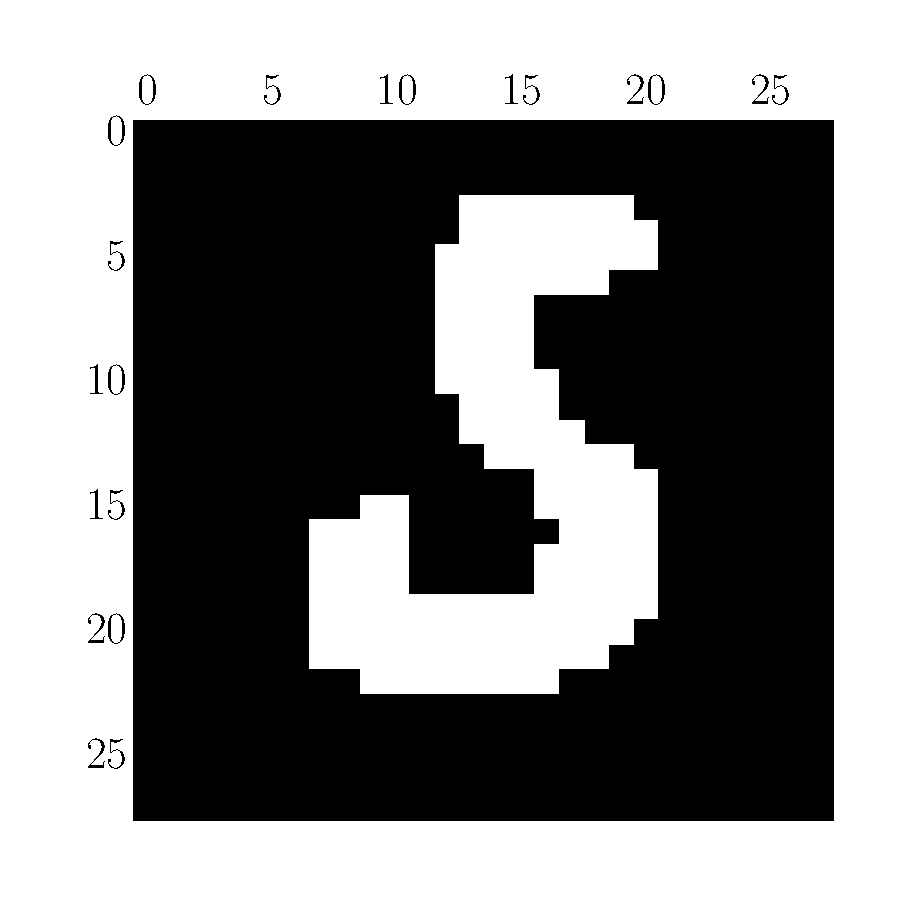
\includegraphics[scale=0.5]{error_50_10_whiletrue.pdf}
\caption{A representative of the few examples in tha data set hard to learn. In this case a 5 was very often mistaken for a 3 in several run of both the linear and the RBF Gaussian kernel batch mode algorithm.}
\label{default}
\end{center}
\end{figure}

\begin{figure}[htbp]
\begin{center}
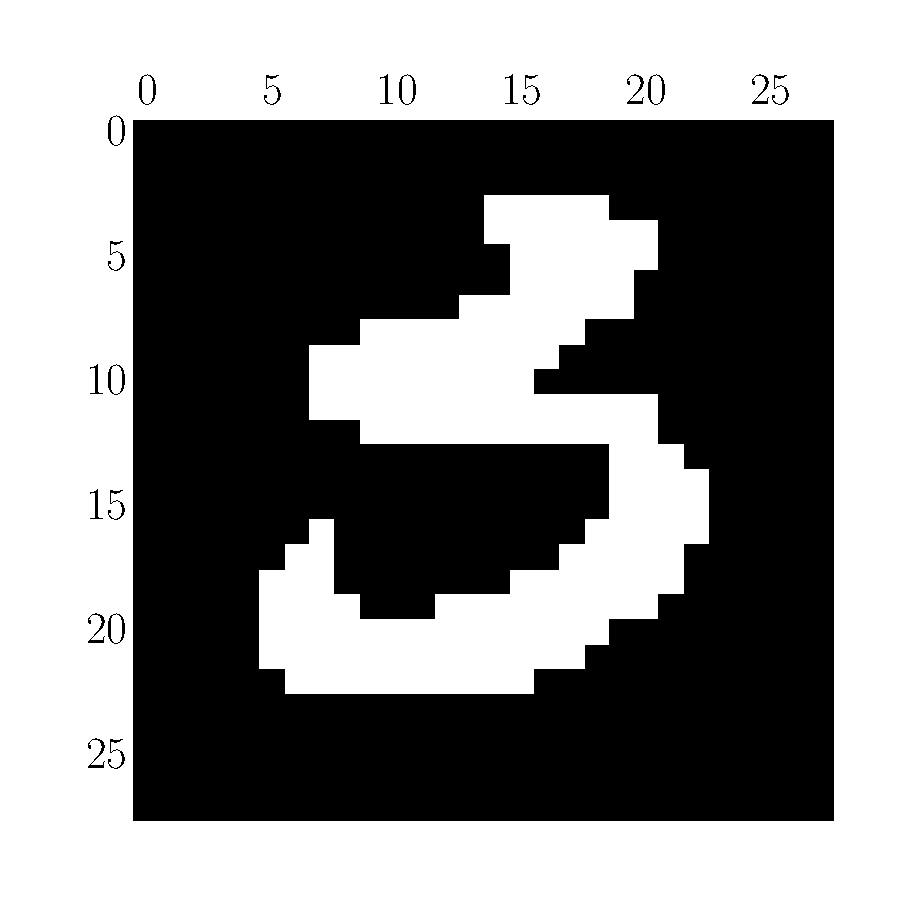
\includegraphics[scale=0.5]{error_1312_10_whiletrue.pdf}
\caption{A representative of the few examples in tha data set hard to learn. In this case a 3 was very often mistaken for a 5 in several run of both the linear and the RBF Gaussian kernel batch mode algorithm.}
\label{default}
\end{center}
\end{figure}

\begin{figure}[htbp]
\begin{center}
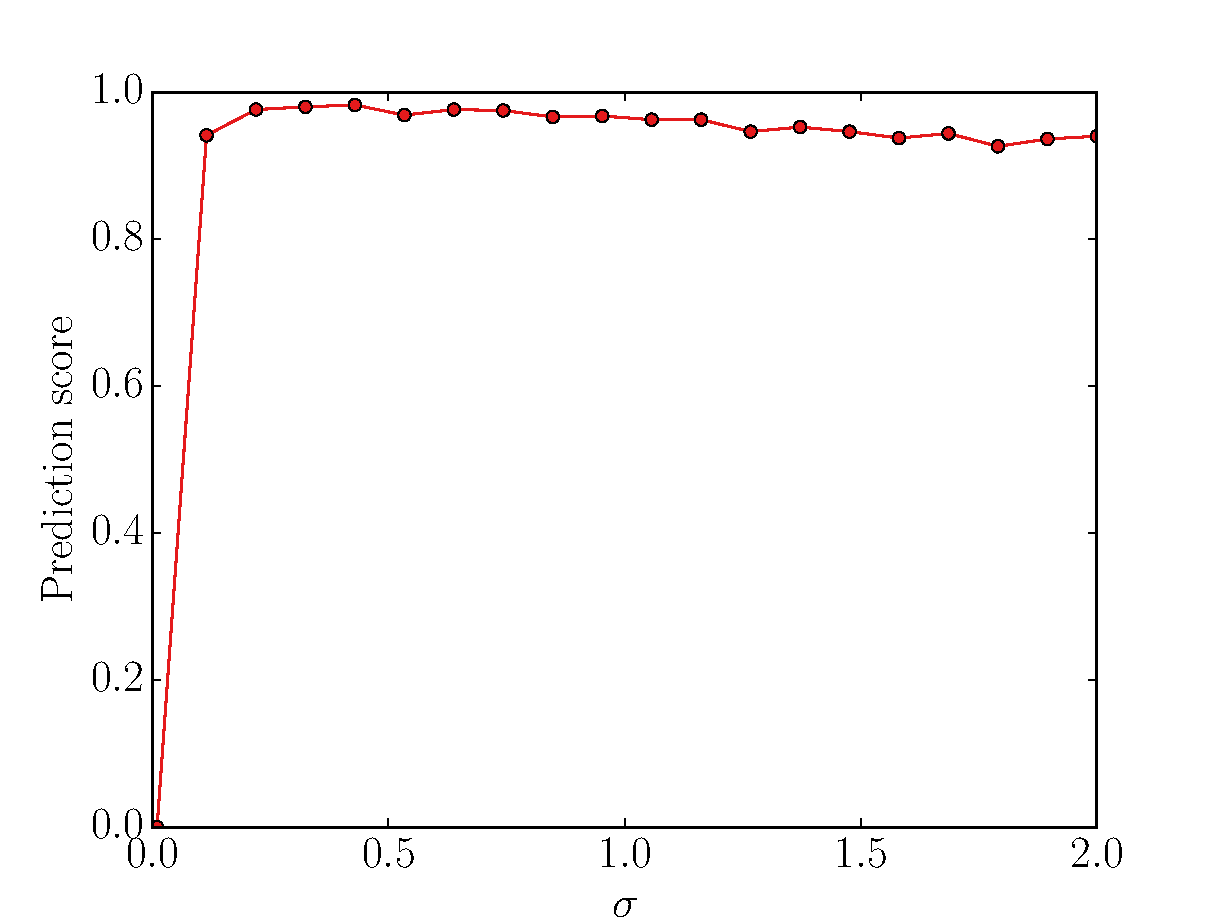
\includegraphics[scale=0.5]{pred_score3.pdf}
\caption{First of 3 different scales example of my training of the sigma parameter in the RBF kernel. I held $40\%$ of the dataset off from the training one and then tested the accuracy on that. I did not perform more advanced cross validation trying to held different part of the dataset etc.
\underline{The performance seems to be quite flat in $\sigma$ for a significant range}. Slightly decreasing from 0.4 to 2. This was tested with 200 runs of the batch version of the algorithm.
}
\label{def}
\end{center}
\end{figure}

\begin{figure}[htbp]
\begin{center}
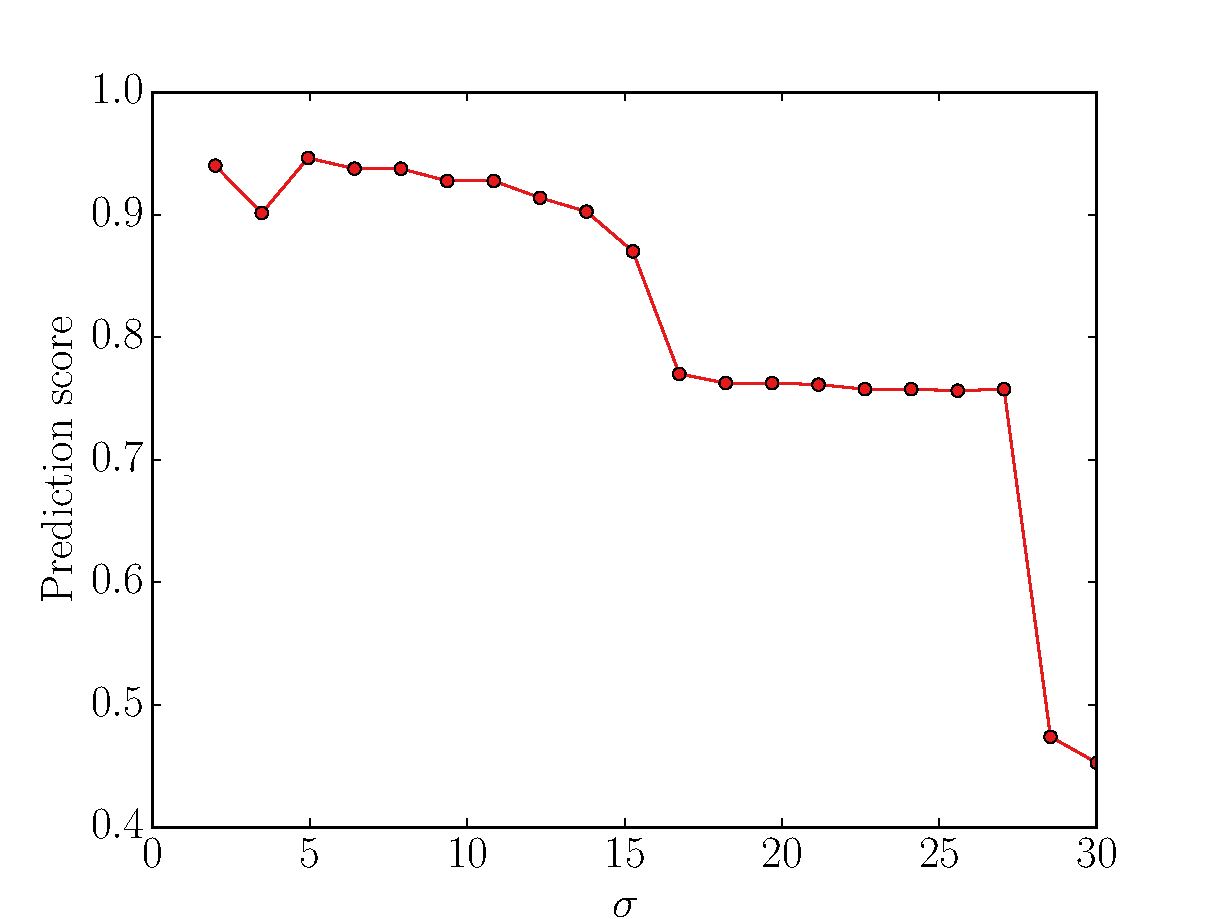
\includegraphics[scale=0.5]{pred_score2.pdf}
\caption{Training of the sigma parameter in the RBF kernel. I held $40\%$ of the dataset off from the training one and then tested the accuracy on that.
\underline{This is an example of the secrease in performance once $\sigma$ became too big ($>10$).}This was tested with 200 runs of the batch version of the algorithm.
}
\label{default}
\end{center}
\end{figure}


\begin{figure}[htbp]
\begin{center}
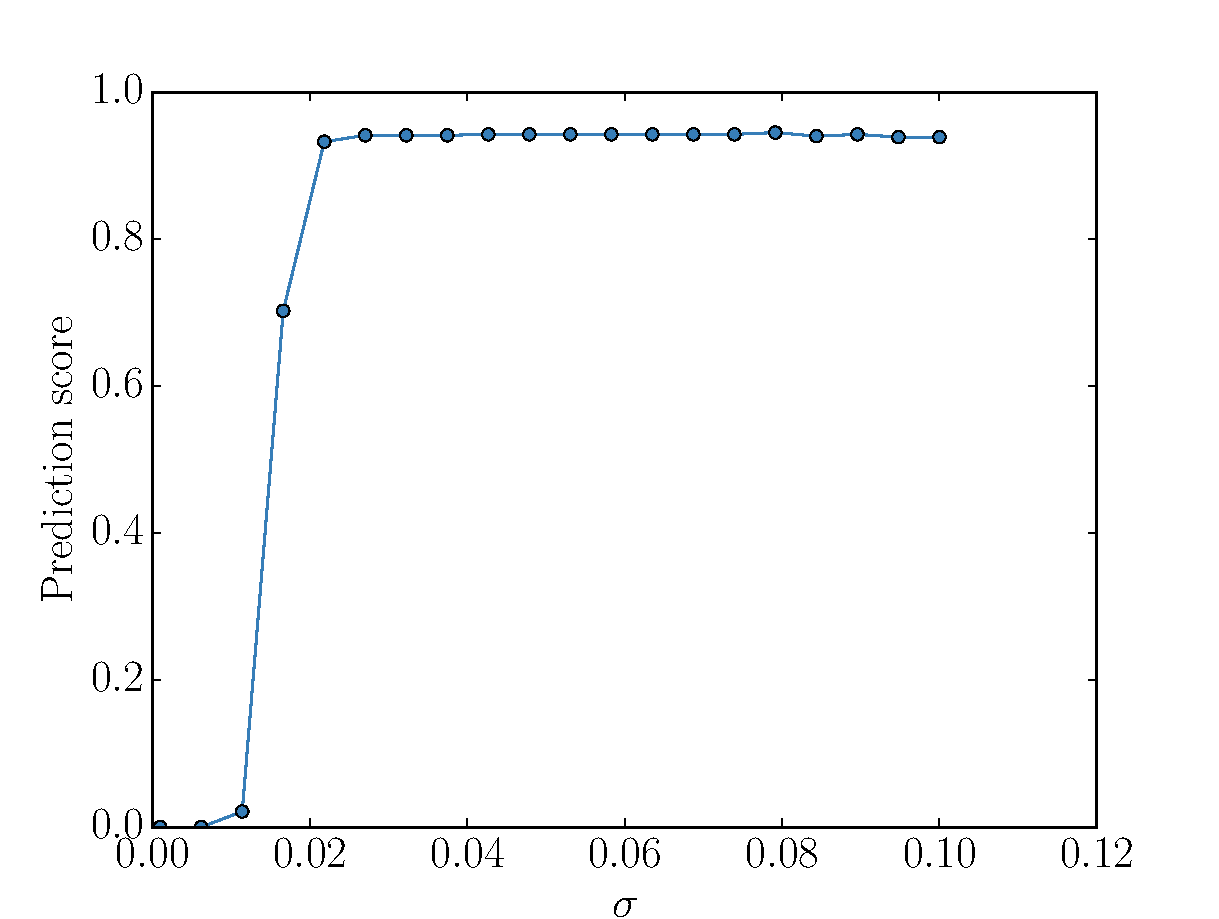
\includegraphics[scale=0.5]{pred_score.pdf}
\caption{Training of the sigma parameter in the RBF kernel. I held $40\%$ of the dataset off from the training one and then tested the accuracy on that.
A zoom in the lowest end of $\sigma$. Smaller than 0.02 seems to be too small. This was tested with 200 runs of the batch version of the algorithm.
}
\label{default}
\end{center}
\end{figure}



\begin{figure}[htbp!]
\begin{center}
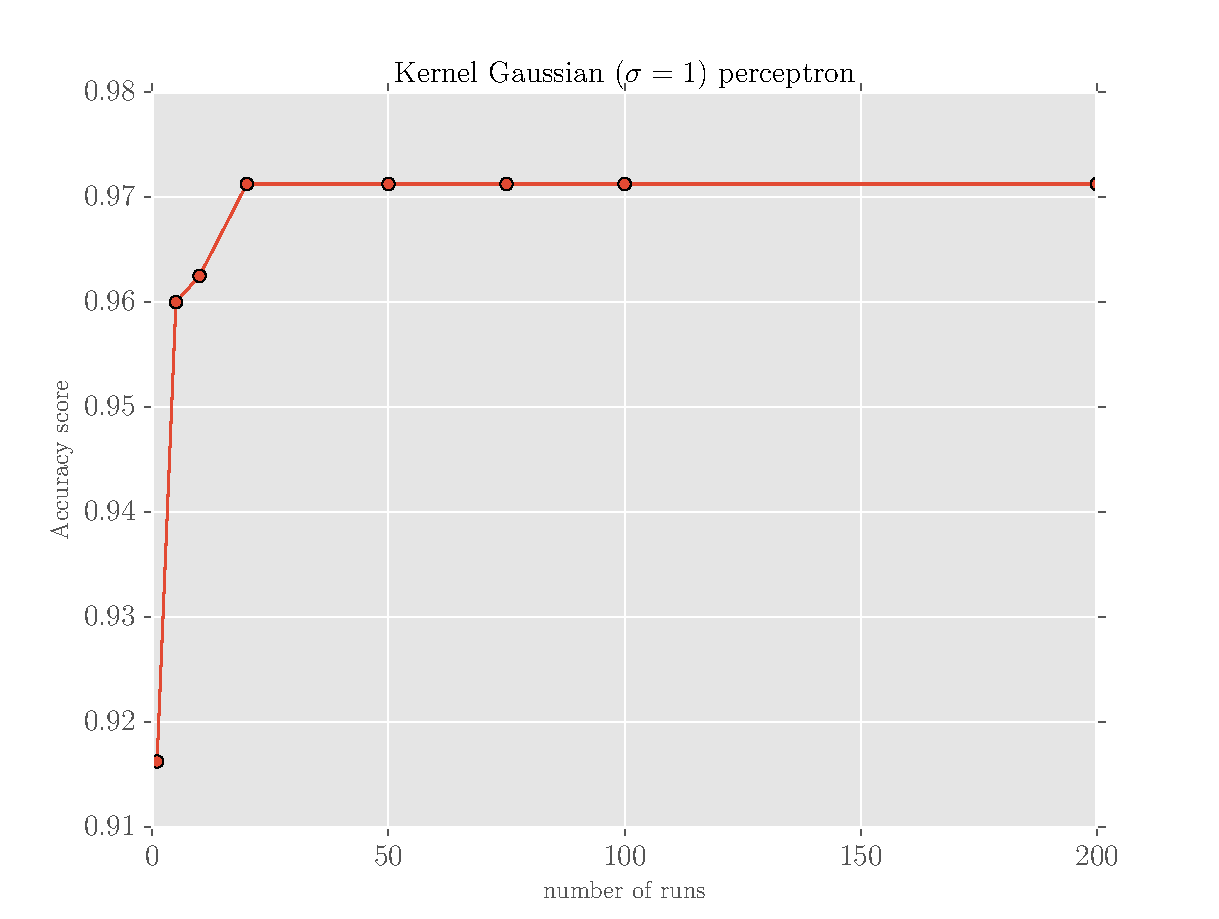
\includegraphics[scale=0.5]{score_run_gaussian.pdf}
\caption{Gaussian. Quick test of the performances as a function of number of times the algorithm is run in batch mode.}
\label{default}
\end{center}
\end{figure}

\begin{figure}[htbp!]
\begin{center}
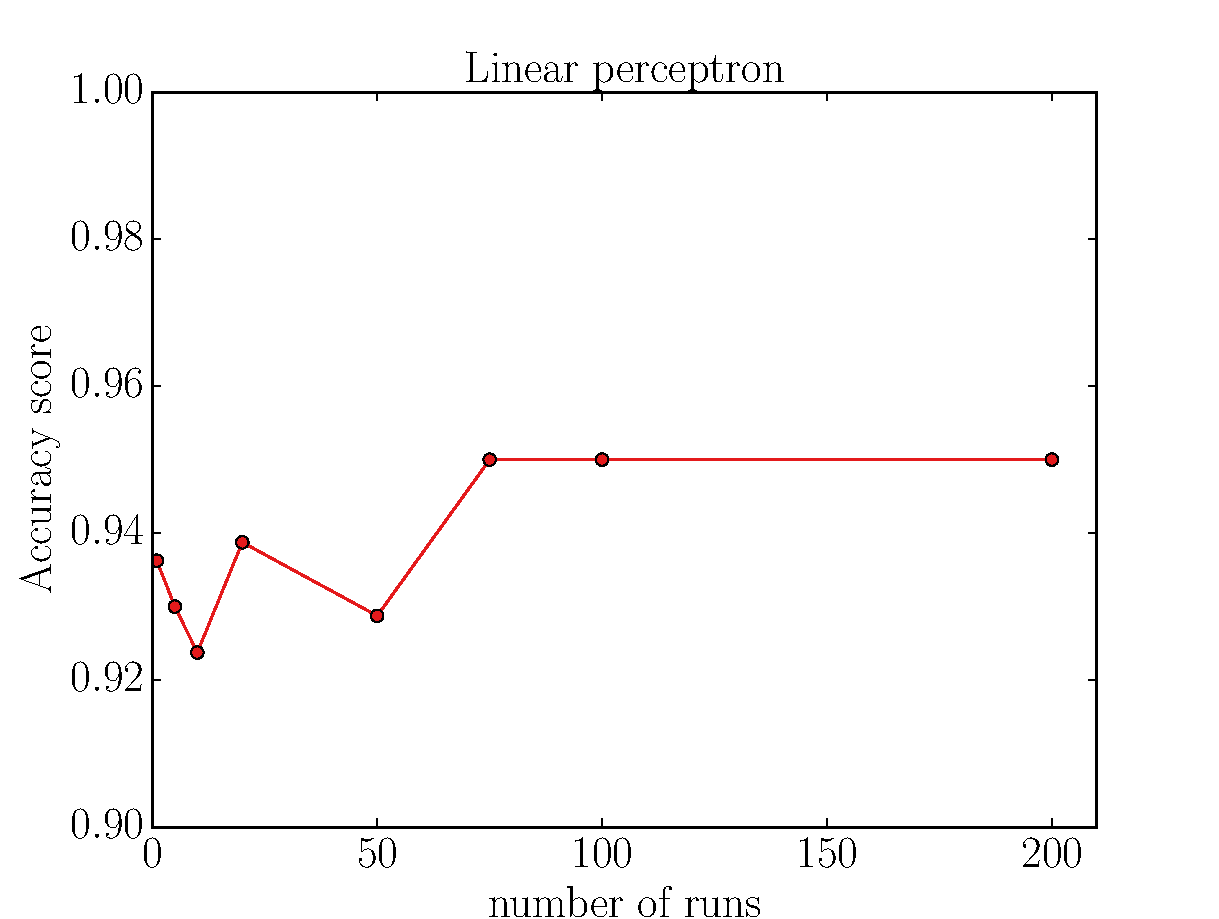
\includegraphics[scale=0.5]{score_run_liner.pdf}
\caption{Linear. Quick test of the performances as a function of number of times the algorithm is run in batch mode.}
\label{default}
\end{center}
\end{figure}



\section{Problem 2}
\begin{description}
\item[Code] All is done in \texttt{gaussian\_processes.py}
\end{description}


\begin{figure}[htbp!]
\begin{center}
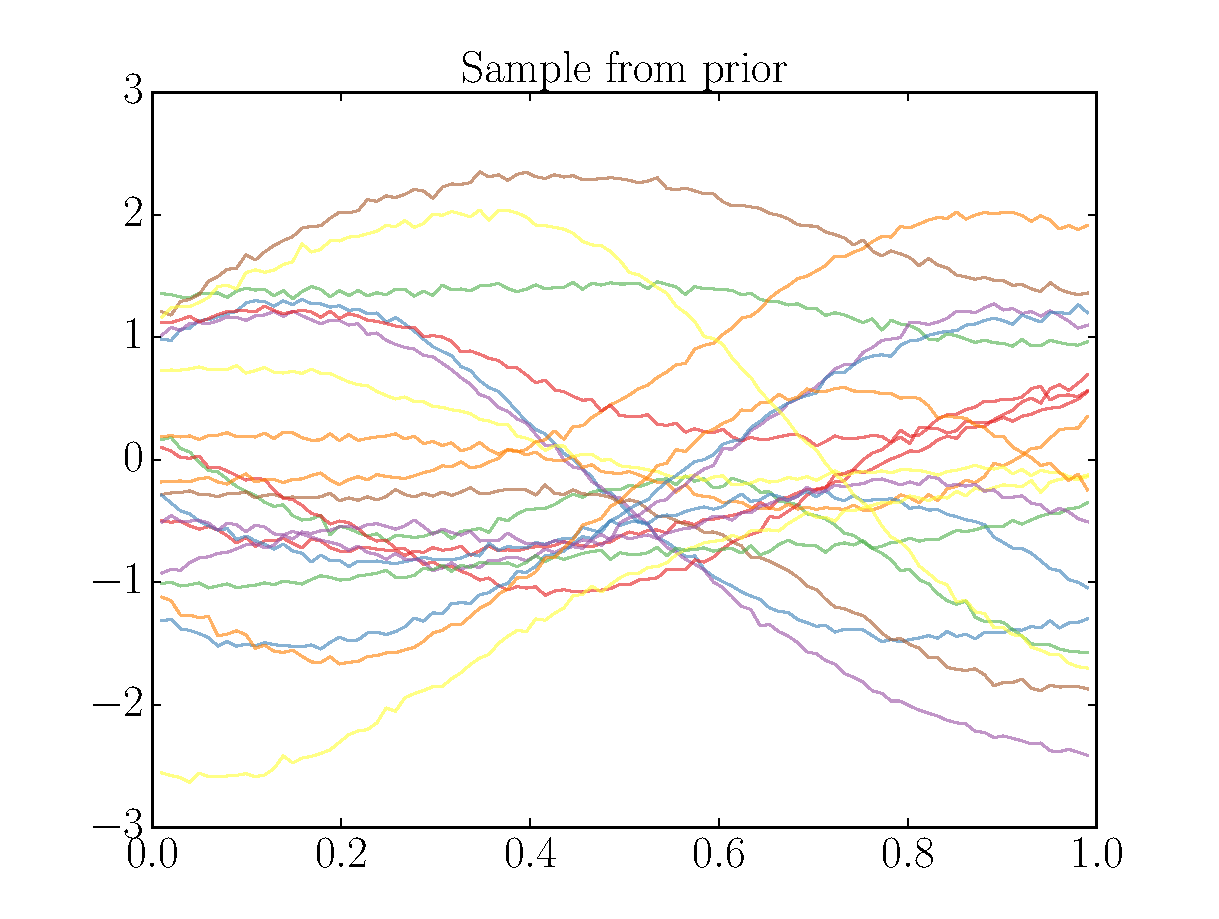
\includegraphics[scale=0.5]{sample_prior_2.pdf}
\caption{2a. Example of 20 fucntions draw from the $G(\mu,k)$ prior. This was done using the iterative procedure suggested in the HW text.
I needed to add a small $1e5$ regularization factor to K and avoid inverting the K matrix directly to avoid numerical instabilities while using a lot of (very close) points.}
\label{default}
\end{center}
\end{figure}


\begin{figure}[htbp!]
\begin{center}
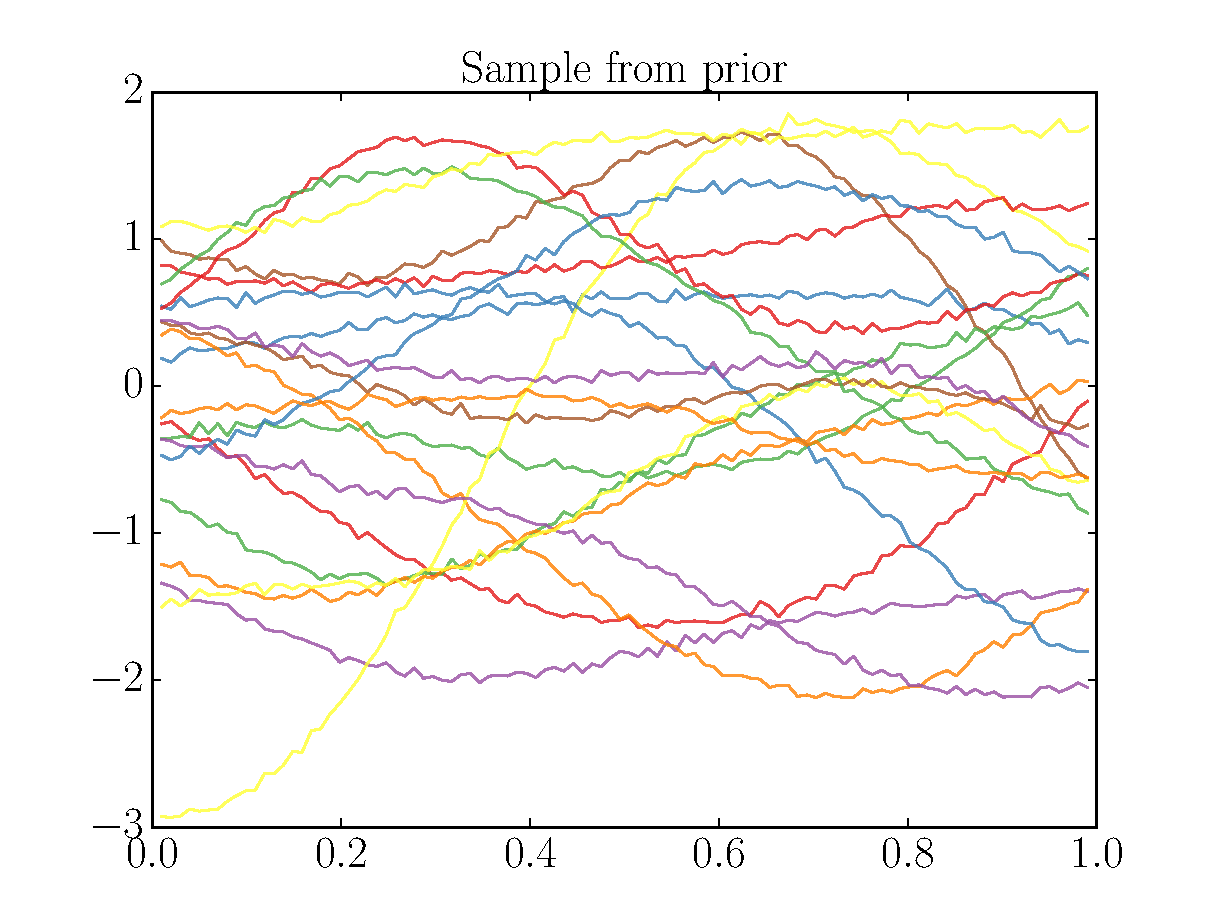
\includegraphics[scale=0.5]{sample_prior.pdf}
\caption{2a. Example of 20 fucntions draw from the $G(\mu,k)$ prior. This was done sampling from a multivariate gaussian with mean zero and covariance k using native \texttt{numpy} functions}
\label{default}
\end{center}
\end{figure}




\begin{figure}[htbp!]
\begin{center}
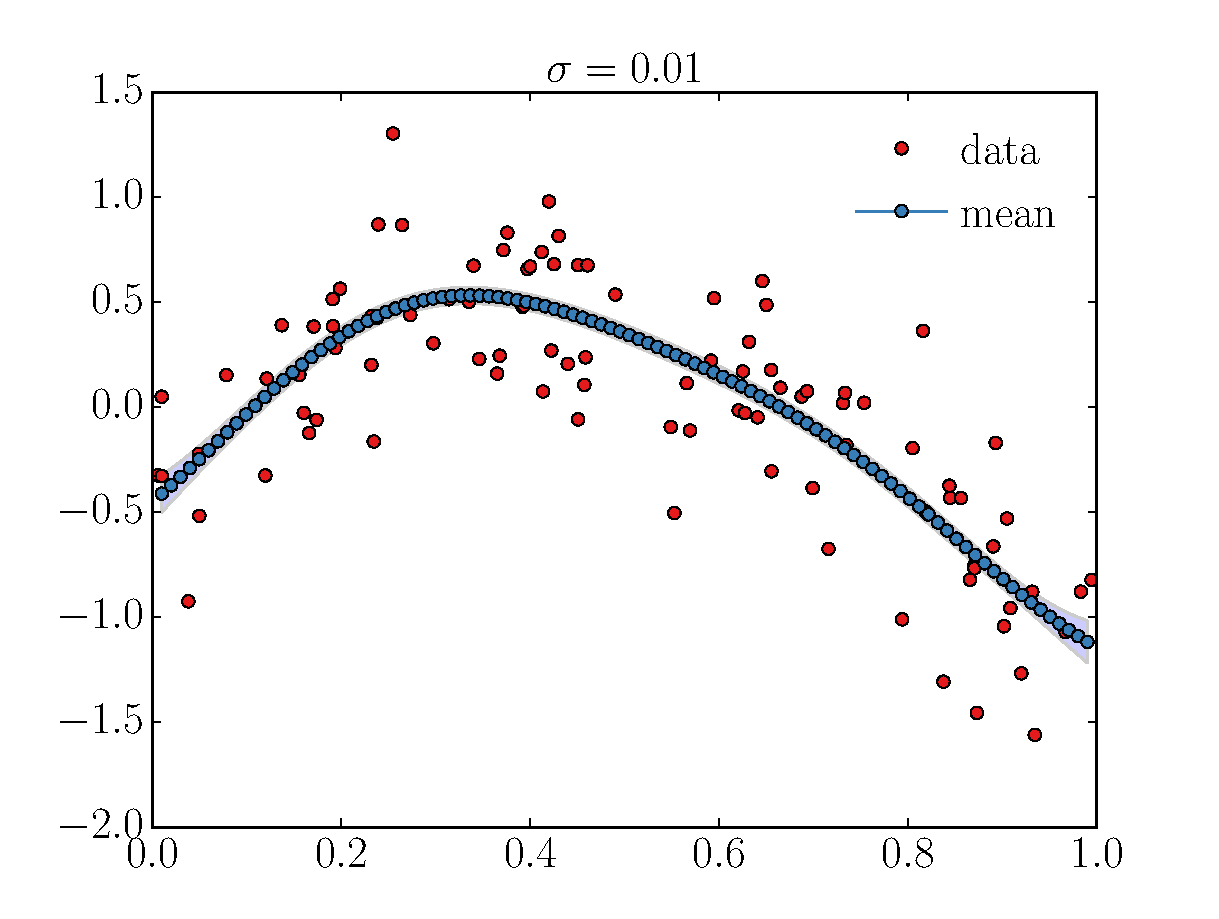
\includegraphics[scale=0.5]{fig3.pdf}
\caption{2b. Posterior mean and 2 standard deviation bound for different choices of the parameter $\sigma$. The data are also plotted.}
\label{default}
\end{center}
\end{figure}

\begin{figure}[htbp!]
\begin{center}
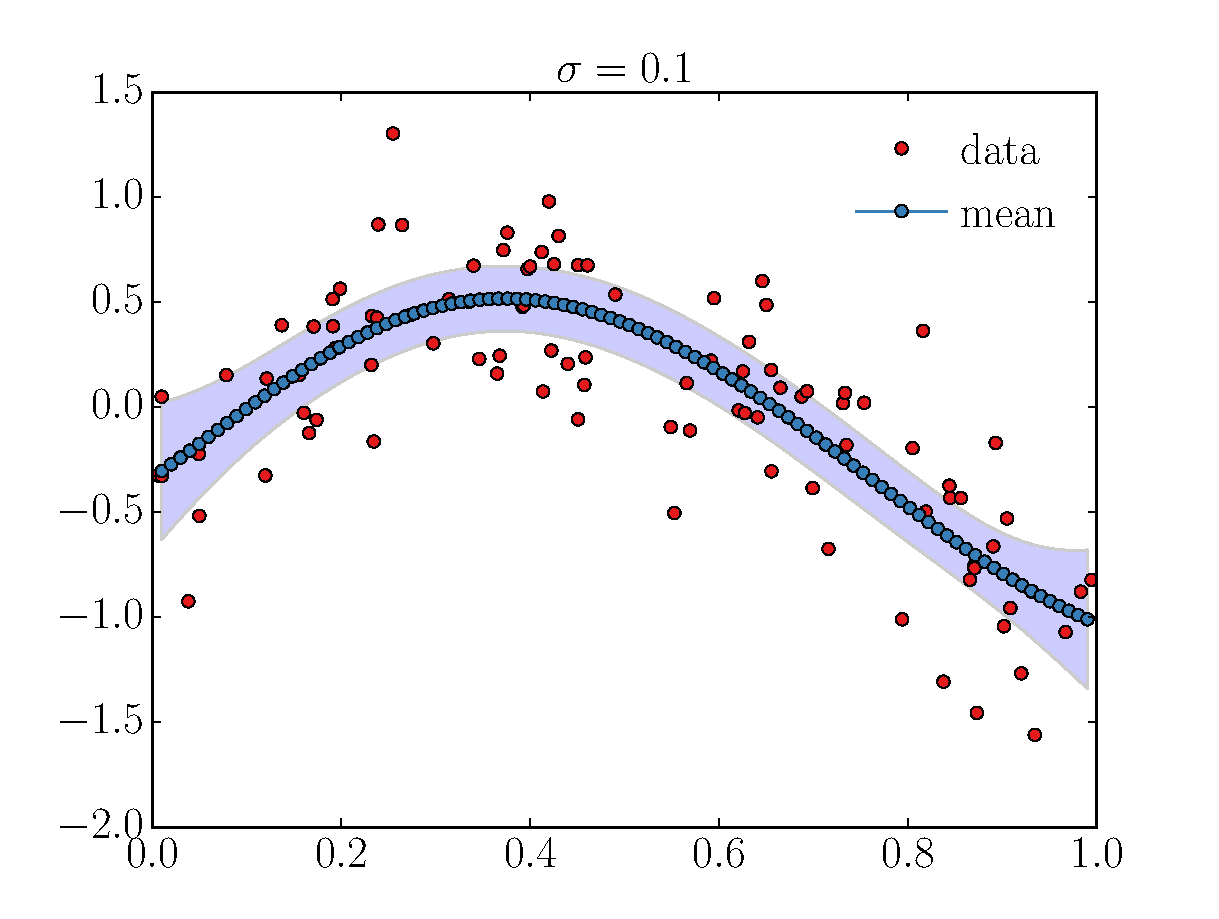
\includegraphics[scale=0.5]{fig2.pdf}
\caption{2b. Posterior mean and 2 standard deviation bound for different choices of the parameter $\sigma$. The data are also plotted.}
\label{default}
\end{center}
\end{figure}

\begin{figure}[htbp]
\begin{center}
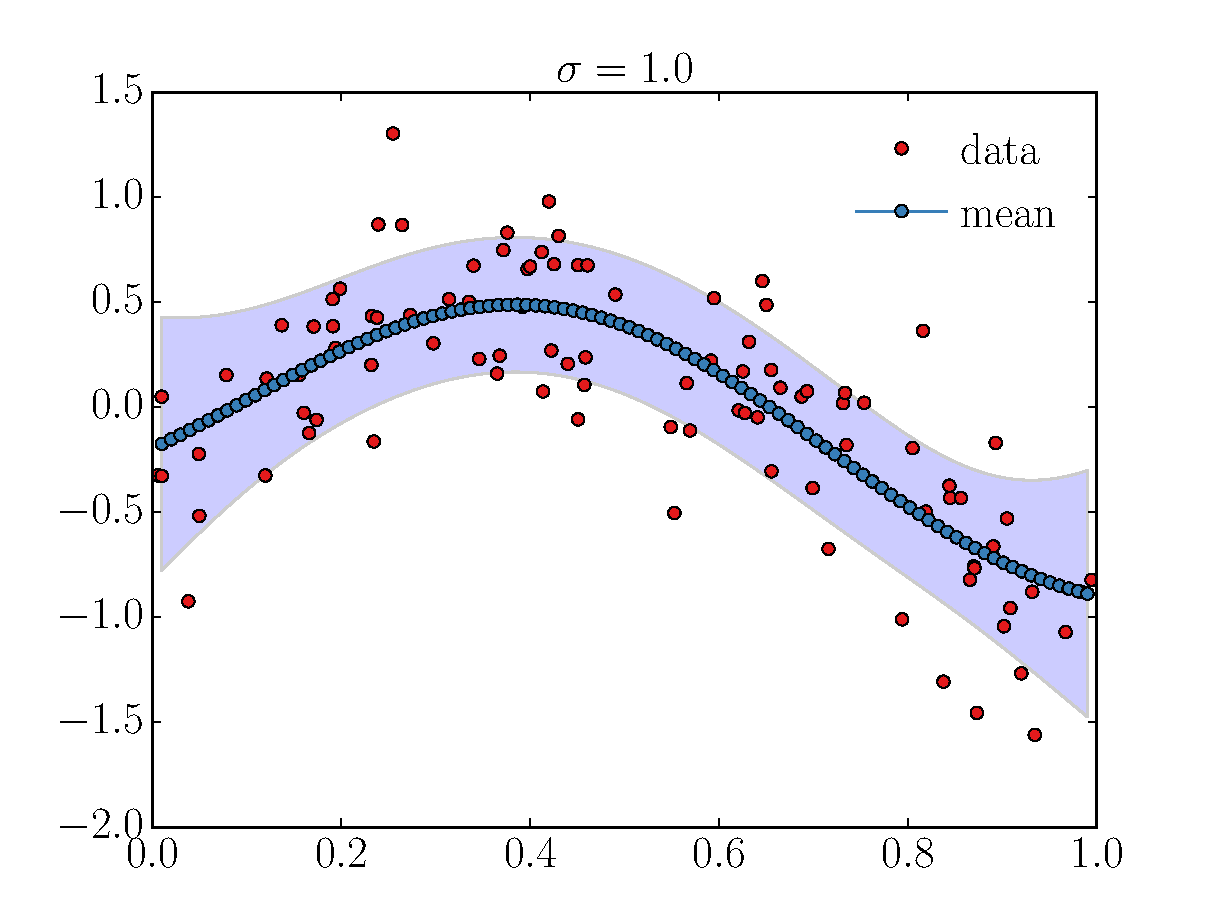
\includegraphics[scale=0.5]{fig1.pdf}
\caption{2b. Posterior mean and 2 standard deviation bound for different choices of the parameter $\sigma$. The data are also plotted.}
\label{default}
\end{center}
\end{figure}

\begin{figure}[htbp]
\begin{center}
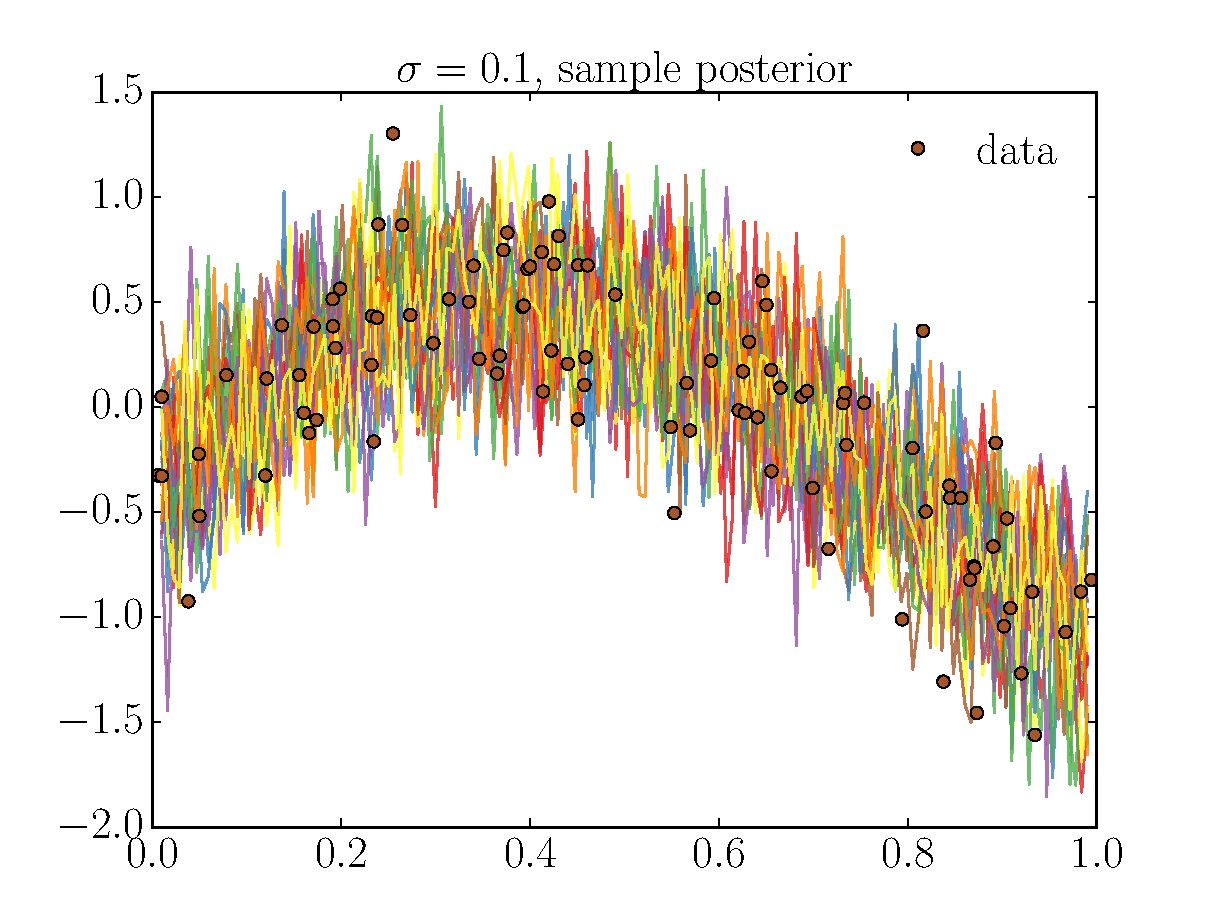
\includegraphics[scale=0.5]{sample_posterior01.pdf}
\caption{2c. 20 functions sampled from the posterior. This example was for $\sigma=0.1$}
\label{default}
\end{center}
\end{figure}

\begin{figure}[htbp]
\begin{center}
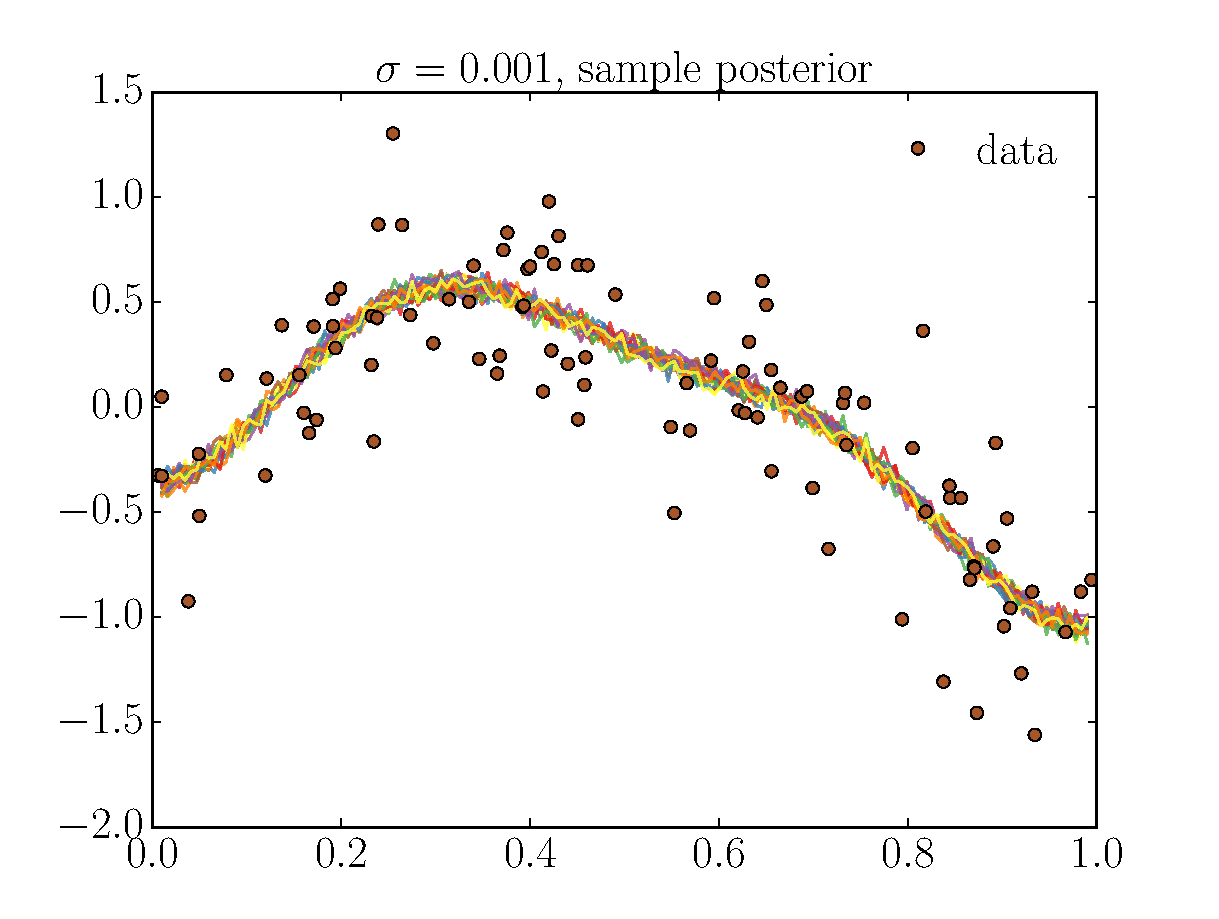
\includegraphics[scale=0.5]{sample_posterior0001.pdf}
\caption{2c. 20 functions sampled from the posterior. This example was for $\sigma=0.001$. Assuming a small noise in the data force the sampled curves to stay close to the mean.\underline{ Not sure if there is an optimal value for $\sigma$}. \underline{By eye the sigma seems to be close to $0.1-1$}. However given the value of $\tau$ in the kernel the functions are pretty rapidly oscillating and basically picking up noise if $\sigma>0.01$}
\label{default}
\end{center}
\end{figure}


\end{document}